In p-multigrid, the different grids have the same number and size of finite elements but with different order basis functions.
The grid transfer operators can be represented elementwise and can thus be easily represented in the form of Equation \ref{eq:libceed_representation}.

The prolongation operator from the coarse to the fine grid interpolates low-order basis functions at the nodes for the high-order basis functions.
Figure \ref{fig:p_prolongation} shows the evaluation of second order basis function on the Gauss-Lobatto nodes for a fourth order basis.
This basis evaluation operation will be extended for LFA of h-multigrid and BDDC.

\begin{figure}[!ht]
  \centering
  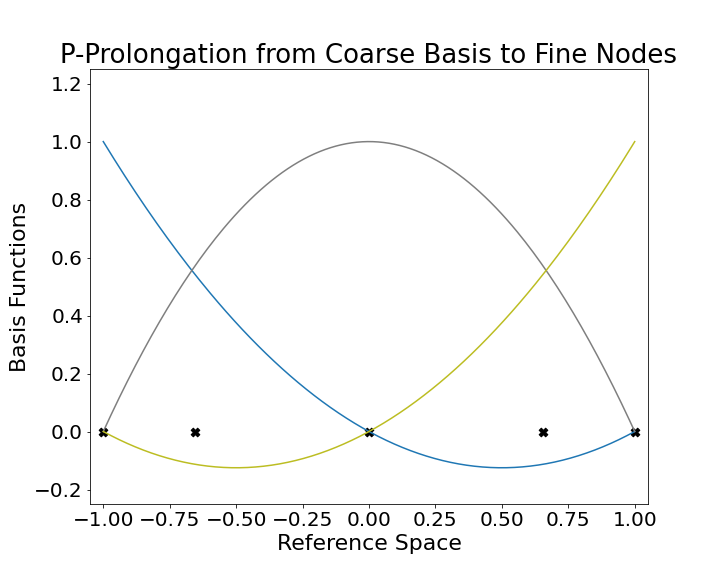
\includegraphics[width=0.48\textwidth]{../img/pProlongation}
  \caption{P-Prolongation from Coarse Basis to Fine Basis Points}
  \label{fig:p_prolongation}
\end{figure}

With this coarse to fine basis interpolation, the prolongation operator can be be represented by
\begin{equation}
\begin{tabular}{c}
${\color{burgundy}\mathbf{P}}_{\text{ctof}} = \mathbf{P}_f^T \mathbf{G}_f^T {\color{burgundy}\mathbf{P}}_e \mathbf{G}_c \mathbf{P}_c$\\
${\color{burgundy}\mathbf{P}}_e = {\color{blue(ncs)}\mathbf{I}} {\color{applegreen}\mathbf{D}}_{\text{scale}} {\color{blue(ncs)}\mathbf{B}}_{\text{ctof}}$
\end{tabular}
\end{equation}
where ${\color{blue(ncs)}\mathbf{B}}_{\text{ctof}}$ is an interpolation operator from the coarse grid basis to the fine grid basis, $\mathbf{P}_f$ and $\mathbf{G}_f$ are the fine grid element assembly operators, $\mathbf{P}_c$ and $\mathbf{G}_c$ are the coarse grid element assembly operators, and ${\color{applegreen}\mathbf{D}}_{\text{scale}}$ is a scaling operator to account for node multiplicity across element interfaces.
Restriction from the fine grid to the coarse grid is given by the transpose, ${\color{burgundy}\mathbf{R}}_{\text{ftoc}} = {\color{burgundy}\mathbf{P}}_{\text{ctof}}^T$.

It is useful to think of the p-prolongation operation as an interpolation operation between the coarse and fine grids, but in practice it can be easier to construct the prolongation basis ${\color{blue(ncs)}\mathbf{B}}_{\text{ctof}}$ from the coarse and fine grid interpolation operators, provided that both bases use the same quadrature space.
\begin{equation}
\begin{tabular}{c c}
${\color{blue(ncs)}\mathbf{B}}_f = \mathbf{Q} \mathbf{R},$ & ${\color{blue(ncs)}\mathbf{B}}_{\text{ctof}} = \mathbf{R}^{-1} \mathbf{Q}^T {\color{blue(ncs)}\mathbf{B}}_c$
\end{tabular}
\label{eq:p_prolong_basis}
\end{equation}
In Equation \ref{eq:p_prolong_basis}, we form the interpolation operation between the coarse grid from the coarse grid interpotation operator and the QR factorization of the fine grid interpolation operator.
Note that in the case of H1 Lagrange bases, this factorization will produce the same coarse to fine grid interpolation operator as evaluating the coarse grid basis functions at the fine grid nodes.

Following the derivation from Section \ref{sec:lfahighorder}, we can derive the symbols of ${\color{burgundy}\mathbf{P}}_{\text{ctof}}$ and ${\color{burgundy}\mathbf{R}}_{\text{ftoc}}$.

\begin{definition}
The symbol of the p-prolongation operator is given by
\begin{equation}
\tilde{{\color{burgundy}\mathbf{P}}}_{\text{ctof}} \left( \theta \right) = \mathbf{Q}_f^T \left( {\color{burgundy}\mathbf{P}}_e \odot \left[ e^{\imath \sum_d \left( \mathbf{x}_{i, f} - \mathbf{x}_{j, c} \right) \mathbf{\theta} / \mathbf{h}} \right] \right) \mathbf{Q}_c
\end{equation}
where $i \in \left[ 0, 1, \dots, \left( p_{\text{fine}} \right)^{\text{dim}} \right]$, $h$ is the length of the element, and $j \in \left[ 0, 1, \dots, \left( p_{\text{coarse}} \right)^{\text{dim}} \right]$.
The matrices $\mathbf{Q}_f$ and $\mathbf{Q}_c$ are the localization mappings for the fine and coarse grid, respectively, and the element p-prolongation operator is given by ${\color{burgundy}\mathbf{P}}_e = {\color{blue(ncs)}\mathbf{I}} {\color{applegreen}\mathbf{D}}_{\text{scale}} {\color{blue(ncs)}\mathbf{B}}_{\text{ctof}}$.
\label{def:p_prolongation_symbol}
\end{definition}

\begin{definition}
The symbol of p-restriction operator is given by the expression
\begin{equation}
\tilde{{\color{burgundy}\mathbf{R}}}_{\text{ftoc}} \left( \theta \right) = \mathbf{Q}_c^T \left( {\color{burgundy}\mathbf{R}}_e \odot \left[ e^{\imath \sum_d \left( \mathbf{x}_{i, c} - \mathbf{x}_{j, f} \right) \mathbf{\theta} / \mathbf{h}} \right] \right) \mathbf{Q}_f
\end{equation}
where $i \in \left[ 0, 1, \dots, \left( p_{\text{coarse}} \right)^{\text{dim}} \right]$, $h$ is the length of the element, and $j \in \left[ 0, 1, \dots, \left( p_{\text{fine}} \right)^{\text{dim}} \right]$.
The matrices $\mathbf{Q}_f$ and $\mathbf{Q}_c$ are the localization mappings for the fine and coarse grid, respectively, and the element p-restriction operator is given by ${\color{burgundy}\mathbf{R}}_e = {\color{burgundy}\mathbf{P}}_e^T = {\color{blue(ncs)}\mathbf{B}}_{\text{ctof}}^T {\color{applegreen}\mathbf{D}}_{\text{scale}} {\color{blue(ncs)}\mathbf{I}}$.
\label{def:p_restriction_symbol}
\end{definition}

\begin{figure}[!ht]
  \centering
  \subfloat[Spectrum of P-Multigrid for $p_f = 4$, $p_c = 2$]{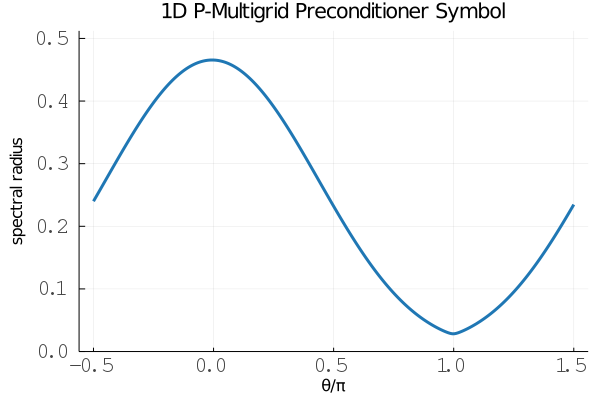
\includegraphics[width=0.48\textwidth]{../img/pmultigridSymbol1D}\label{fig:p_multigrid_spectrum_1d}}
  \hfill
  \subfloat[Spectrum of P-Multigrid for $p_f = 4$, $p_c = 2$]{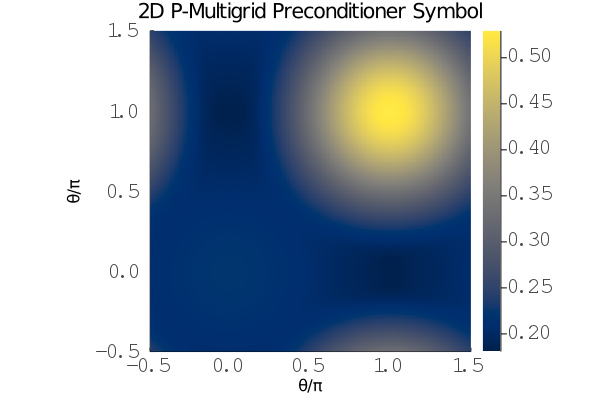
\includegraphics[width=0.48\textwidth]{../img/pmultigridSymbol2D}\label{fig:p_multigrid_spectrum_2d}}
  \caption{Spectrum of Spectrum of P-Multigrid Symbol for $p_f = 4$, $p_c = 2$}
\end{figure}

In Figures \ref{fig:p_multigrid_spectrum_1d} and \ref{fig:p_multigrid_spectrum_2d}, we see the spectral radius of the symbol of p-multigrid for the scalar diffusion operator with third-order Chebyshev smoothing on a fine grid with a fourth-order H1 Lagrange finite element basis and a coarse grid with a second-order H1 Lagrange finite element basis on the Gauss-Lobatto points in one and two dimensions.
Various preconditioning techniques will reduce this spectral radius, with different effectiveness in different frequency ranges.
